\renewcommand{\theequation}{\theenumi}
\begin{enumerate}[label=\arabic*.,ref=\thesubsubsection.\theenumi]
\numberwithin{equation}{enumi}
%
\item Let the man be at point $\vec{M}$ = $\myvec{0\\0}$ \\
The speed of the man is $\vec{u}$ = $\myvec{0\\4}$ \\
The speed of the river is $\vec{v}$ = $\myvec{3\\0}$ \\
Since the swimmer dive the river normal to the flow of river, therefore time taken by swimmer to cross the river, 
$$ t = \frac{d}{\norm{\vec{u}}} = \frac{1 km}{4 km/h} = 15 mins$$

Distance covered down the river = $t \times \norm{\vec{v}}$
$$ x = \frac{1}{4} hr \times 3 km/h = 750 m$$

The code for diagrammatic representation(\ref{fig:triangle1}) of the solution is
\begin{lstlisting}
codes/line/motion_plane/man_river.py
\end{lstlisting}  
\begin{figure}[!ht]
\centering
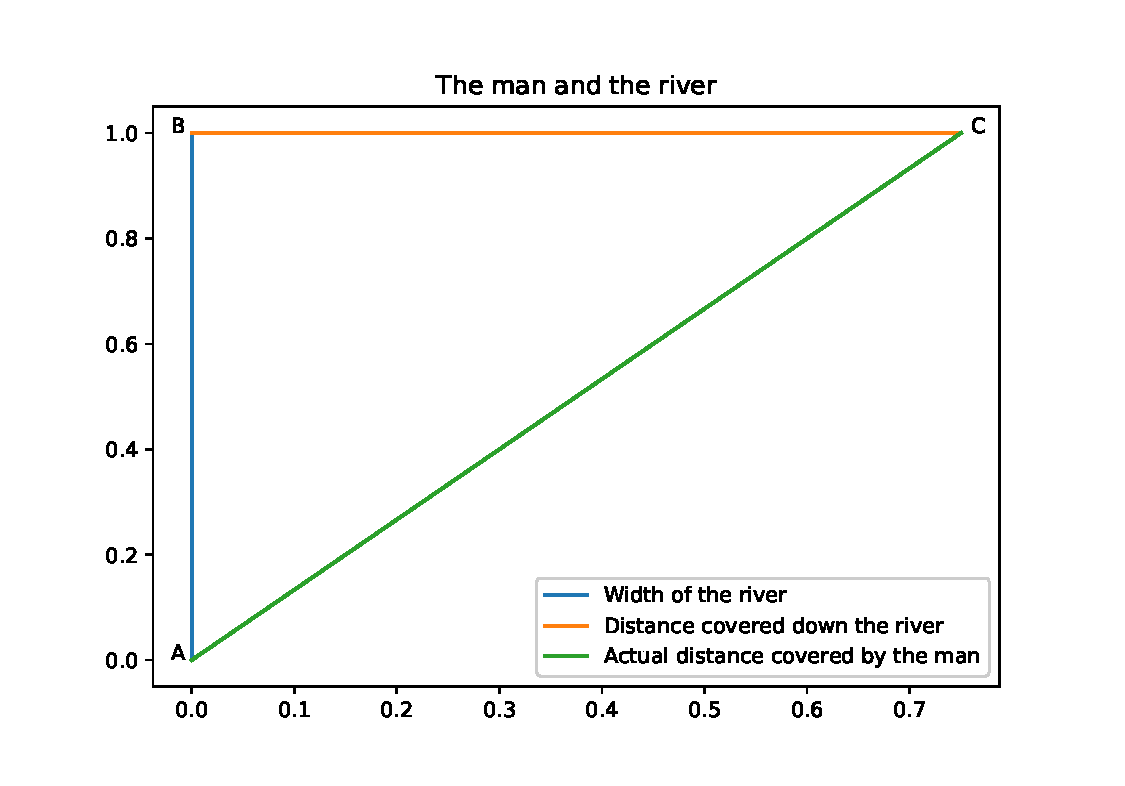
\includegraphics[width=\columnwidth]{./codes/line/motion_plane/man_river.eps}
\caption{}
\label{fig:triangle1}
\end{figure}
\end{enumerate}
